Surface plasmon resonance is remarkably sensitive to perturbations in the bulk
refractive index of the medium in which SPPs propagate.  By monitoring
properties of the notch in the specular direction, sensitivities of up to
\SI{1e-8}{RIU} (refractive index units) have been reported in some
applications~\cite{fan2008sensitive}, shot noise limited.  Bulk refractive
index sensing and its limits are particularly well
understood~\cite{piliarik2009surface}, so this section focuses on similar types
of measurements in the cone.  Effects from speckle are not considered.

In a prism-coupled setup, there are three main methods used to monitor changes
in the SPR resonance condition.  All three of these interrogation methods are
equivalent in terms of their real-world resolution and detection
limit~\cite{homola2006surface}.
\begin{description}
\item [{Angular}] The change in the angle of the SPR minimum as a function
of refractive index is monitored.  In the angular modulation method,
the prism may be scanned through a range of angles or the angular
spectrum may be obtained simultaneously using a focused beam and
sensor array.
\item [{Wavelength}] The prism is fixed in place and its reflectivity at
a single angle is monitored as a function of wavelength.
\item [{Intensity}] For a fixed wavelength and incident angle, the
intensity of the signal at a certain angular or spatial point is
monitored as the experiment progresses.
\end{description}
This section is restricted to analysis in the angular and intensity
interrogation methods.  The experimental setup does not possess the means to
carry out wavelength interrogation, though this is in many ways equivalent to
sweeping the SPR angle.

\subsection{Angular Interrogation}
To study the sensitivity in the angular interrogation method, the angular
response of the system was simulated using the Fresnel equations with ($\Delta
n = 0$) and without ($\Delta n \ne 0$) a refractive index perturbation of the
sensing layer.  An example is shown in \Figure{fig:sensangularasp} for both
conventional and long-range SPPs.  The choice of $\Delta n = 0.01$ is somewhat
arbitrary and was made to illustrate the change of the resonance line.
Notwithstanding, the SPR resonance shifts in response to a refractive index
perturbation.

In the simulation, the minimum of the SPR resonance was determined using
nonlinear minimization~\cite{brent1973algorithms} and optimizing the function
as $\Delta n \to 0$.  In this way, the maximum theoretical sensitivity for
angular sensitivity, $\Delta \theta/\Delta n$ is determined.  This theoretical
sensitivity should not be confused with real world sensitivity; sources of
noise in the experiment and detector are not taken into account.  Nor is the
present analysis concerned with optimization of sensitivity, rather it is most
relevant to ascertain the difference between angular response to refractive
index perturbations in the cone and the notch.
\begin{figure}[ht]
\centering
\import{includes/}{setpgfinc}
\import{bulkri/figures/}{sens_angular_asp}
\import{bulkri/figures/}{sens_angular_ssp}
\caption{(top) Angular sensitivity of the notch and the cone for the
	Kretschmann three-layer (SP) system.
	$\lambda_0=\SI{660}{\nano\meter}$, $n_1 = \num{1.5142}$,
	$n_2=\num{0.2843 + 3.3825i}$, and $n_3=1.3310 + \Delta n$.  The
	thickness of the metal layer is \SI{45}{\nano\meter}. (bottom) Angular
	sensitivity of the notch and the cone for the Kretschmann four-layer
	(LRSPP) system.  $\lambda_0=\SI{660}{\nano\meter}$, $n_1
	= \num{1.5142}$, $n_2=1.3489$, $n_3=\num{0.2843 + 3.3825i}$, and
	$n_4=1.3310+\Delta n$.  The thickness of the metal layer is
	\SI{16.97}{\nano\meter}.  }
\label{fig:sensangularasp}
\end{figure}
In compliment to \Figure{fig:sensangularasp}, the maximum obtainable
sensitivities for these configurations are tabulated in
\Table{tbl:angularsens}.  The tabulated data supports the hypothesis that
there is no readily apparent sensitivity benefit to the cone versus the notch
in angular interrogation.  Though the angle of the SPR minima (notch) and
maxima (cone) are at slightly different angles, approximately
\SI{0.006}{\degree}, their responses track each other very well.

\begin{table}[ht]
\centering
\sisetup{round-mode=places,round-precision=3,fixed-exponent=0,scientific-notation=fixed}
\begin{tabular}{lSS}
\toprule
{configuration} & {notch [$\mathrm{deg}/\mathrm{RIU}]$} & {cone [$\mathrm{deg}/\mathrm{RIU}$]} \\
\midrule
SP & 1.452312e+02 & 1.453671e+02 \\
LRSPP& 3.943097e+01 & 3.938117e+01 \\
\bottomrule
\end{tabular}
\caption{Theoretical maximum angular sensitivity, $\Delta \theta/\Delta n$, in
	degrees per refractive index unit, for the configurations in
	\Figure{fig:sensangularasp}.}
\label{tbl:angularsens}
\end{table}

\subsection{Intensity Interrogation}

In contrast to angular interrogation, intensity interrogation shows
differences between the notch and the cone, most likely due to both the
sharper resonance and narrower linewidth in the cone.  For the systems under
discussion, the angular width of the notch was determined to be
$\theta_{1/2}=\SI{8.0708}{\degree}$ for conventional surface plasmons, with
the cone being nearly twice as narrow at $\theta_{1/2}=\SI{4.7795}{\degree}$.
Long-range surface plasmons show the same trend, but the discrepancy is not
nearly as large with $\theta_{1/2}=\SI{0.2349}{\degree}$ for the notch and
$\theta_{1/2}=\SI{0.2325}{\degree}$ for the cone.  The theoretically predicted
maximum sensitivities for both cases are shown in \Table{tbl:intensitysens}.
The tabulated data was obtained using the same nonlinear minimization method
as for angular case, but the calculation instead sought the angular location where the
difference in Fresnel coefficients is maximized as $\Delta n \to 0$.
Specifically, for an $N$ layer system with refractive indices $(n_1,n_2,
\ldots,n_N)$,
\begin{equation}
\lim_{\Delta n \to 0}\frac{\left||r^p(n_N=n_N)|^2 - |r^p(n_N=n_N + \Delta
				n)|^2\right|_\mathrm{max}}{\Delta n}.
\label{eqn:fresnelsenspertrubation}
\end{equation}
For the cone, the same approach was used but instead of the Fresnel
reflectivity, \Equation{eqn:conefield}, $|t^p_+|^2|t^p_-|^2$.  In
both cases the signal is normalized to $[0,1]$ within the same angular range
for comparison.

The results of are summarized in
\Table{tbl:intensitysens}.  In both cases it is observed $\Delta I/\Delta
n$ is higher for the cone as compared with the notch, though the increase
is only marginal.  In terms of SPR biosensors, the difference suggests an
avenue for sensitivity enhancement, though whether implementing such a
strategy is warranted in commercial systems remains to be seen.
\begin{table}[ht]
\centering
\sisetup{round-mode=places,round-precision=3,fixed-exponent=0,scientific-notation=fixed}
\begin{tabular}{lSS}
\toprule
{configuration} & {notch [1/RIU]} & {cone [1/RIU]} \\
\midrule
SP & 32.1657 & 42.3053 \\
LRSPP & 203.5365 & 251.9765 \\
\bottomrule
\end{tabular}
\caption{Theoretical maximum intensity sensitivity, $\Delta I/\Delta n$,
								for the configurations in \Figure{tbl:angularsens}. }
\label{tbl:intensitysens}
\end{table}

\section{Refractive Index Effect On Speckle}
\begin{figure}[ht]
\centering
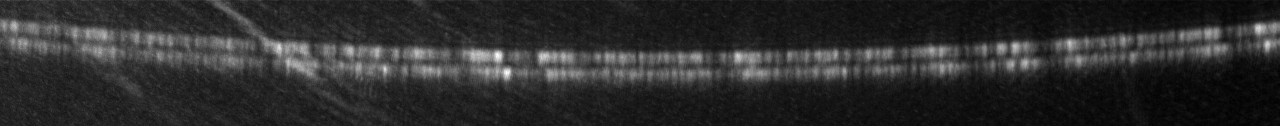
\includegraphics[keepaspectratio,width=15cm]{bulkri/figures/combineri.png}
\caption{Combined cone images of a sample without (top, $\Delta n = 0$) and
with (bottom, $\Delta n = 0.01$) a refractive index pertrubation. }
\label{fig:speckleridrangos}
\end{figure}

To gauge the effect of a refractive index pertrubation on cone speckle,
glucose solutions of varying concentrations were introduced into the
microfluidic flow cell after \SI{57}{\micro\meter} AuNPs had been adsorbed on
to the sensor as in \Section{sec:specklesizeexpf}.

A \SI{10}{\percent} glucose solution was prepared and small amounts of water
added until its refractive index as measured by a water-cooled Abbe
refractometer was $n=1.341$ at \SI{20}{\celsius}.  The refractive index of
deionized water was likewise measured at $n=1.331$.  The combination of these
two liquids amounted to a refractive index pertrubation of $\Delta n = 0.01$.
The liquids were introduced into the microfluidic flow cell, deionized water
first, and the resulting speckle patterns measured as the experiment
progressed.

The primary results of this investigation are depicted in
\Figure{fig:speckleridrangos}.  Here, two subsequent cone images without (top
cone, $\Delta n = 0$, deionized water) and with (bottom cone, $\Delta n =
0.01$, glucose) a refractive index pertrubation are shown as one --- the
images have been added together.  The addition of the two images is
straightforward as the position of the cone on the sensor shifts along with
the pertrubation, as is expected.  As can be seen without numerical analysis,
the structure of the speckle is not appreciably different between the two
cases.

The cone images were unwrapped as described in \Section{sec:spkline} and
compared using a one-dimensional average of their azimuthal speckle intensity.
At the extreme of $\Delta n = 0.01$, the Pearson product moment correlation
coefficent, (see \Equation{eqn:pearsonproductmoment} and surrounding
discussion) which has a value of 1 for perfectly correlated signals, reached a
minimum value of $0.9262$, and was naturally higher during the transition from
$\Delta n = 0$ to $\Delta n = 0.01$.

From the measurements it is apparent that small refractive index perturbations
have little effect on the structure of speckle in this setup.  In the next
chapter it will be seen that the underlying scattering microstructure, not
refractive index, is the most sensitive and determining factor concerning
speckle.  In terms of speckle, decorrelation is expected to occur when the
average SPP scattering path undergoes a phase shift of $2\pi$ --- difficult to
realize at this level.

